%!TEX root = ../proposal-presentation.tex

\begin{frame}[c] \frametitle{1. Test Data}

	\textbf{Aim: to have appropriate data for development}

	\vfill

	For initial development:

	\begin{itemize}\itemsep10pt
		\item Publicly available RGB-D datasets
		\item \cite{firman2016}
	\end{itemize}

	\vfill

	For embodied testing:

	\begin{itemize}\itemsep10pt
		\item Create at least one physical scene
	\end{itemize}

	\missingfigure{Example image(s)}

	\vfill

\end{frame}


\begin{frame}[c] \frametitle{2. Object Discovery on Single Images}

	\textbf{Aim: to be able to accurately detect objects in a static image}

	Saliency-based system \cite{garcia2013computational}

\end{frame}


\begin{frame}[c] \frametitle{3. Determining the Next Best View}

	\textbf{Aim: to be able to calculate the viewing which maximises information gain}

	But...

	\begin{itemize}
		\item Limited energy
		\item Limited time
	\end{itemize}

	Possible implementations:

	\begin{itemize}
		\item Subsumption architecture \cite{brooks1986robust}
		\item Information gain \cite{surmann2003autonomous}
		\item POMDPs \cite{lauri2015planning}
	\end{itemize}

	\vfill

	\textbf{Question:} update while the robot is moving?

\end{frame}


\begin{frame}[c] \frametitle{4. Fusing Multiple Views}

	\textbf{Aim: to be able to create a 3D model from multiple images}

	\medskip

	\begin{enumerate}

		\item Solve SLAM problem

		\begin{itemize}\itemsep10pt
			\item FastSLAM
			\item RatSLAM
			\item \ldots
		\end{itemize}

		\medskip

		\item Fuse 2D images to 3D model

		\begin{itemize}\itemsep10pt
			\item KinectFusion
		\end{itemize}

		\vfill

		\centering
		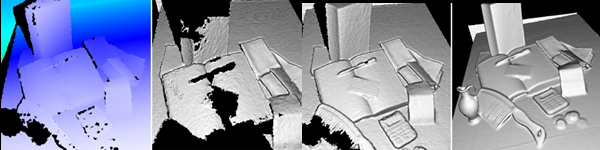
\includegraphics[width=.8\linewidth]{src/kinectfusion.png}

	\end{enumerate}



\end{frame}


\begin{frame}[c] \frametitle{5. Moving the Robot}

	\textbf{Aim: to be able to move the robot to a specific point}

	\bigskip

	% \begin{itemize}
	% 	\item ROS
		\begin{itemize}\itemsep10pt
			\item \texttt{MoveBaseAction}
			\item \texttt{actionlib}
		\end{itemize}
	% \end{itemize}

	\vfill

	
\includegraphics[width=0.8\linewidth]{src/ros.png}

	\vfill

\end{frame}


\begin{frame}[c] \frametitle{6. System Evaluation}

	\textbf{Aim: optimisation and comparison}

	\begin{itemize}\itemsep10pt
		\item Find optimal parameters
		\item Compare different approaches
		\item Compare to previously published approaches
	\end{itemize}

\end{frame}
